\documentclass[12pt]{article}

\usepackage[a4paper, margin=1in]{geometry}
\usepackage{fancyhdr}
\usepackage{titling}
\usepackage{babel}[latvian]
\usepackage{graphicx}
\usepackage{float}


\fancypagestyle{plain}{
  \fancyhf{}
  \fancyhead[R]{ Andrejs Cvečkovskis \\ ac24005 \\ Kurss Zinātniskā programmēšana fiziķiem}
  \renewcommand{\headrulewidth}{0pt}
}

\title{\vspace{-1cm}\centering Laboratorijas darba \\[1ex] \large Pandas \\ Protokols \vspace{-6em}}
\author{}
\date{}  
\begin{document}
\maketitle

\section*{1. nodarbība.}

\subsection*{1. uzdevums.} Uzrakstīt kodu, kas visos trīs veidos piekļūst Annas vecumam. Kāda vērtība tiek izvadīta? \\

 \noindent\textbf{Atbilde:} Visos trīs gadījumos tiek izvadīta vērtība \textbf{21}.
     \\

\noindent \textbf{Piezīme:} \begin{verbatim}
    print(cilveki.iloc[1, 1])
    print(cilveki.loc['Anna', 'vecums'])
    print(cilveki.vecums[1])
    \end{verbatim}

\subsection*{2. uzdevums.} Izvēlēties tās novērojumu stacijas, kuru ģeogrāfiskais garums (lon) ir starp 24 un 26 un kuras atrodas augstumā zem 50 metriem. Kādas un cik loģiskās operācijas tiek izmantotas?\\

\noindent \textbf{Atbilde:} Tiek izmantotas divas salīdzinošās operācijas un viena loģiskā (AND) operācija, kas apvieno šos divus nosacījumus. 
        \begin{table}[ht]
                    \centering
                    \begin{tabular}{ccccc}
                    \hline
                     & station & lon & lat & elevation \\ \hline
                    0  & Ainazi  & 24.3660 & 57.8679 & 6.28 \\
                    2  & Bauska  & 24.1829 & 56.4158 & 30.18 \\
                    13 & Riga    & 24.1161 & 56.9506 & 6.15 \\
                    17 & Skulte  & 24.4122 & 57.3006 & 7.66 \\ \hline
                    \end{tabular}
                    \label{tab:stationdata}
                    \end{table}

\noindent \textbf{Piezīme:} \texttt{stacijas[(stacijas.lon>24)*(stacijas.lon<26)*(stacijas.elevation<50)]}


\subsection*{3. uzdevums.}
    \begin{enumerate}
        \item Rokgrupas ‘Queen’ solists Fredijs Merkūrijs piedzima 1946. gada 5. septembrī un mira 1991. gada 24. novembrī. Izmantojot pandas pieejamās iespējas, aprēķini, cik dienas nodzīvoja Fredijs Merkūrijs.\\

        \textbf{Atbilde:} 16516.0\\

        \textbf{Piezīme:} \begin{verbatim}
birth = pd.to_datetime("1946-09-05 00:00:00")
death = pd.to_datetime("1991-11-24 00:00:00")
print((death-birth)/pd.Timedelta(days=1))
        \end{verbatim}  
        
        \item Izmantojot \texttt{pandas} pieejamās iespējas noteikt nedēļas dienu, kurā piedzima Fredijs Merkūrijs. Noteikt gan konkrēto dienu, gan tās indeksu.\\

        \textbf{Atbilde:} 3; 1946-09-05 00:00:00\\

        \textbf{Piezīme:} \begin{verbatim}
birth_date = pd.to_datetime('1946-09-05 00:00:00')
date = pd.to_datetime(birth_date)
print(birth_date.dayofweek)
print(date)
        \end{verbatim}      
        
        \item Izmantojot pandas iespējas, nosaki, kurš laika moments ir vēlāks: \newline 2023. gada 9. februāris 19:00 pēc Ņujorkas, ASV (America/New York) laika vai 2023. gada 10. februāra 06:00 pēc Šanhajas, Ķīna (Asia/Shanghai) laika. Pārveidot abus uz Latvijas laiku (Europe/Riga).\\

        \textbf{Atbilde:} 2023. gada 9. februāris 19:00 pēc Ņujorkas ir vēlāks.\newline New York: 2023-02-10 02:00:00+02:00 \newline Shanghai: 2023-02-10 00:00:00+02:00\\
        \textbf{Piezīme:} \begin{verbatim}
new_york_time = pd.to_datetime
("2023-02-09 19:00:00").tz_localize('America/New_York', ambiguous=False)
shanghai_time = pd.to_datetime
("2023-02-10 06:00:00").tz_localize('Asia/Shanghai', ambiguous=False)

print(new_york_time > shanghai_time)
print(new_york_time < shanghai_time)
print(new_york_time.tz_convert('Europe/Riga'))
print(shanghai_time.tz_convert('Europe/Riga'))
        \end{verbatim}

        \item 2021 gada 2. februārī es nopirku jaunu datoru, kuram garantijas ilgums ir 1000 dienas. Izmantojot \texttt{pandas} iespējas, noteikt datumu, kad datoram beidzās garantija.\\
        \textbf{Atbilde:} 2023-10-30 00:00:00\\
        \textbf{Piezīme:} \begin{verbatim}
buy_date = pd.to_datetime('2021-02-02 00:00:00')
dt = pd.Timedelta(days=1000)
exp_date = (buy_date+dt)
print(exp_date)
        \end{verbatim}
    \end{enumerate}

\subsection*{4. uzdevums.} Izmantojot \texttt{loc} piekļūt temperatūrai 2010. gada 15. februārī 11:00 pēc Etc/GMT-2 laika zonas.\\

\noindent \textbf{Atbilde:} T = -5.4$^{\circ}$C\\

\noindent \textbf{Piezīme:}
\begin{verbatim}
timestamp = pd.Timestamp('2010-02-15 11:00+02:00').tz_convert(df.index.tz)
temp_2010 = df.loc[timestamp]
print(temp_2010)
\end{verbatim}

\subsection*{5. uzdevums.}
    \begin{enumerate}
        \item Par sala dienu sauc dienu, kad minimālā gaisa temperatūra ir zem 0C. Aprēķināt un uzzīmēt, kā sala dienu skaits ir mainījies pa gadiem.\\

        \textbf{Atbilde:} 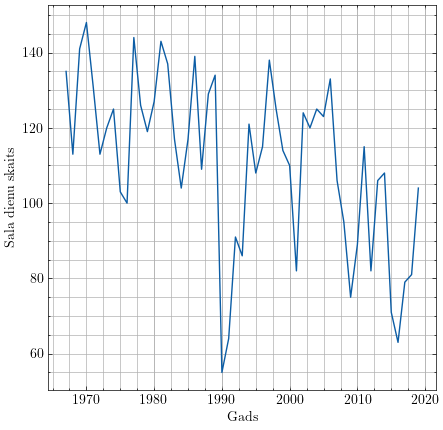
\includegraphics[width=0.5\textwidth]{1.uzd.png}\\

        \textbf{Piezīme:}
        \begin{verbatim}
df2 = df.resample('d').min()
df2 = df2[df2.values<0]
df2 = df2.resample('y').count()
            
plt.figure(figsize=(5,5))
plt.plot(df2)
plt.grid(which='both')
plt.xlabel('Gads')
plt.ylabel('Sala dienu skaits')
plt.show()
        \end{verbatim}

        \item Aprēķināt un uzzīmēt, kā ir mainījusies vasaras (jūn, jūl, aug) vidējā gaisa temperatūra pa gadiem.\\

        \textbf{Atbilde:} 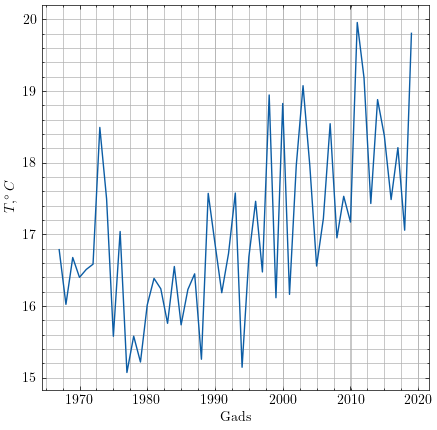
\includegraphics[width=0.5\textwidth]{2.udz.png}\\

        \textbf{Piezīme:}
        \begin{verbatim}
df2 = df[(df.index.month>=6)*(df.index.month<=8)]
df2 = df2.resample('y').mean()

plt.figure(figsize=(5,5))
plt.plot(df2)
plt.grid(which='both')
plt.xlabel('Gads')
plt.ylabel('$T, ^\circ C$')
plt.show()
        \end{verbatim}
        \item Par vasaras dienu sauc dienu, kad maksimālā gaisa temperatūra pārsniedz 25C. Aprēķināt un uzzīmēt, kā vasaras dienu skaits ir mainījies pa gadiem.\\

        \textbf{Atbilde:} 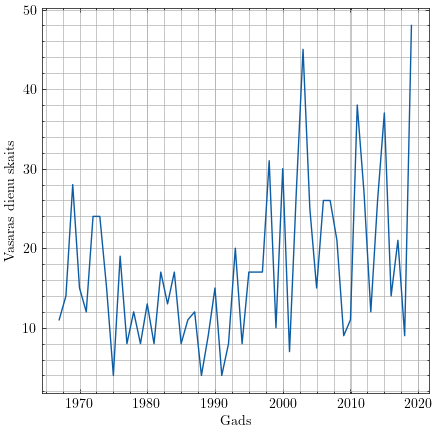
\includegraphics[width=0.5\textwidth]{3.uzd.png}\\

        \textbf{Piezīme:}
\begin{verbatim}
df2 = df.resample('d').max()
df2 = df2[df2.vals>25]
df2 = df2.resample('y').count()

plt.figure(figsize=(5,5))
plt.plot(df2)
plt.grid(which='both')
plt.xlabel('Gads')
plt.ylabel('Vasaras dienu skaits')
plt.show()
\end{verbatim}
        \item Aprēķināt un uzzīmēt, kā ir mainījusies diennakts maksimālās temperatūras vidējā vērtība pa gadiem.\\

        \textbf{Atbilde:} 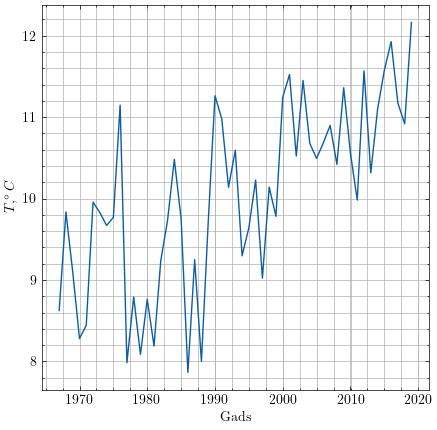
\includegraphics[width=0.5\textwidth]{4. uzd.png}\\

        \textbf{Piezīme:}
\begin{verbatim}
df2 = df.resample('d').max()
df2 = df2.resample('y').mean()

plt.figure(figsize=(5,5))
plt.plot(df2)
plt.grid(which='both')
plt.xlabel('Gads')
plt.ylabel('$T, ^\circ C$')
plt.show()
\end{verbatim}
        \item Izmantojot temperatūras datus no 1970. līdz 2000. gadam katrai gada dienai (dayofyear) aprēķināt vidējo temperatūru, ko sauksim par gaisa temperatūras normu. Uzzīmēt vienā grafikā diennakts gaisa temperatūras normu un katras diennakts vidējo temperatūru 2016. gadā. Aprēķināt, cik dienās gaisa temperatūra bija virs normas un cik dienās zem normas. Ja nepieciešams, pārveidojiet pandas datu masīvus uz numpy datu masīviem. Par garajiem gadiem neuztraukties un vienkārši grupēt pēc dayofyear.\\

        \textbf{Atbilde:} 249 dienās gaisa temperatūra virs normas. \newline 117 dienās gaisa temperatūra zem normas.\\
        \textbf{Piezīme:}
\begin{verbatim}
norma = df[(df.index.year>=1970)*(df.index.year<=2000)]
norma = norma.groupby(norma.index.dayofyear).mean()

gads = df[df.index.year==2016]
gads = gads.groupby(gads.index.dayofyear).mean()

print(int(np.sum(gads>norma)), 'dienās gaisa temperatūra virs normas')
print(int(np.sum(gads<norma)), 'dienās gaisa temperatūra zem normas')

plt.figure(figsize=(10, 5))
plt.plot(norma)
plt.plot(gads)
plt.grid(which='both')
plt.xlabel('Gada diena')
plt.ylabel('$T, ^\circ C$')
plt.legend(['1970-2000 norma', '2016. gads'])
plt.show()
\end{verbatim}
        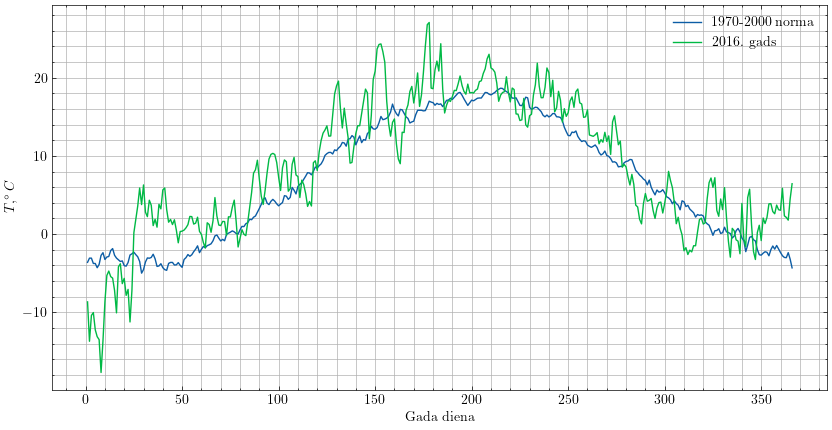
\includegraphics[width=0.9\textwidth]{5.uzd..png}
    \end{enumerate}

\subsection*{6. uzdevums.} Mapē temperatura *.txt failos atrodas temperatūras novērojumu dati no meteoroloģiskajām stacijām visā Latvijā. Izmantojot staciju sarakstu no masīva stacijas, ielasīt datus no visām stacijām un apvienot tās vienā pandas masīvā. To var izdarīt, vispirms ielasot vienas stacijas datus. Tad, ejot ciklā cauri staciju sarakstam, šim masīvam var pievienot pa vienam datus no citām stacijām. Pievienot arī attēlu ar iegūto tabulu.\\

\noindent \textbf{Atbilde:}\\
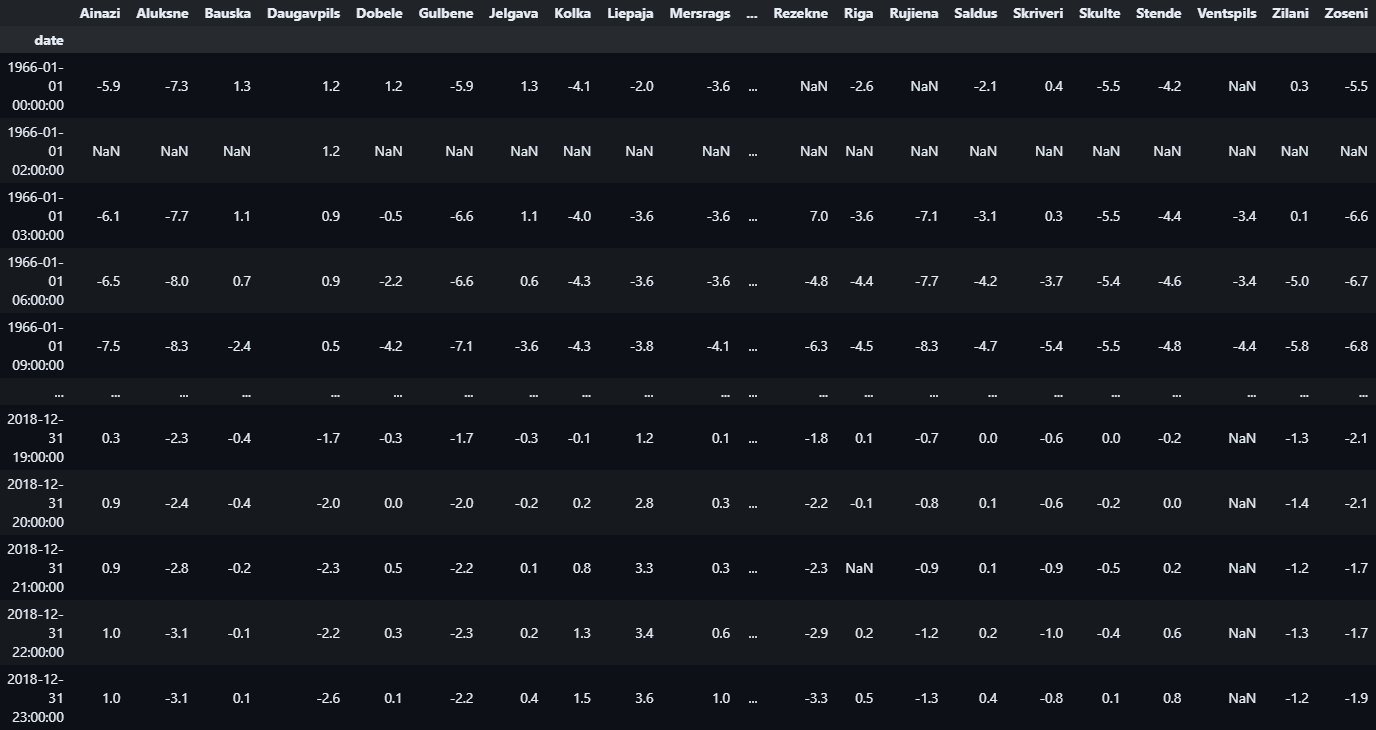
\includegraphics[width=1\textwidth]{6.uzd.png}

\noindent \textbf{Piezīme:}
\begin{verbatim}
df = pd.read_csv('temperatura/Ainazi.txt', sep='\t')
df.set_index('date', inplace=True)
df.index = pd.to_datetime(df.index)
df.columns = ['Ainazi']

for i in range(1, 22):
    df1 = pd.read_csv('temperatura/' + stacijas.station[i] + '.txt', sep='\t')
    df1.set_index('date', inplace=True)
    df1.index = pd.to_datetime(df1.index)
    df1.columns = [stacijas.station[i]]
    
    df = df.join(df1, how='outer')

df = df[(df.index.year>=1966)*(df.index.year<=2018)]

df
\end{verbatim}

\newpage
\section*{2. nodarbība.}

\subsection*{1. uzdevums.} Ielasīt datus, kas glabājas failā taxis.csv, dati failā atdalīti ar komatiem. Piešķirt kolonnām pickup un dropoff datuma formātu. Pataisīt kolonnu pickup kā datu masīva indeksa kolonnu. Pievienot arī attēlu ar iegūto tabulu.\\

\noindent \textbf{Atbilde:} \newline 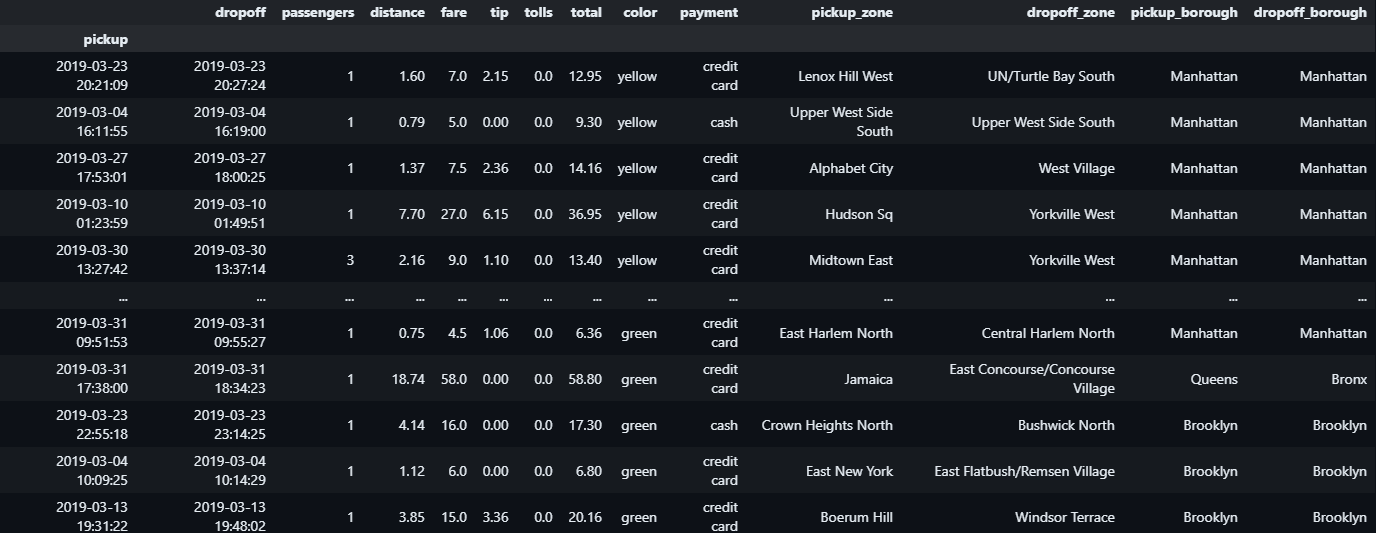
\includegraphics[width=1\textwidth]{1.uzd_2.png}

\noindent \textbf{Piezīme:}
\begin{verbatim}
df = pd.read_csv('taxis.csv', parse_dates=['pickup', 'dropoff'])
df.set_index('pickup', inplace=True)
df
\end{verbatim}

\subsection*{2. uzdevums.} Pievienot datu masīvam kolonnas:
    \begin{enumerate}
        \item Kolonnā \textbf{time} aprēķināt brauciena ilgumu minūtēs.\\
        \textbf{Atbilde:}
        \begin{verbatim}
df['time'] = df.dropoff - df.index
df['time'] = df.time.dt.total_seconds()
df['time_minutes'] = df.time/60
        \end{verbatim}

        \item Kolonnā \textbf{speed} aprēķināt brauciena vidējo ātrumu.\\
        \textbf{Atbilde:}
        \begin{verbatim}
df['mean_speed'] = (df.distance*1000)/(df.time)
        \end{verbatim}
        \item Kolonnā \textbf{fare per kilometer} aprēķināt brauciena izmaksas (fare) uz kilometru\\
        \textbf{Atbilde:}
        \begin{verbatim}
df['fare_per_kilometre'] = df.total/df.distance
        \end{verbatim}
    \end{enumerate}

\subsection*{3. uzdevums.} Izvadīt informāciju par braucienu, kas notika 2019. gada 11. marta 20:45:26. \\
\newline \textbf{Atbilde:} 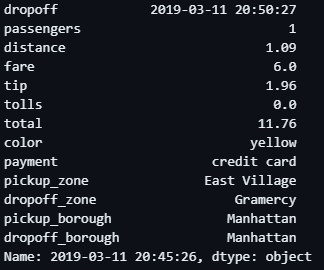
\includegraphics[width=0.5\textwidth]{3.udz.png}

\noindent \textbf{Piezīme:}
\begin{verbatim}
df.loc[pd.to_datetime('2019-03-11 20:45:26')]
\end{verbatim}

\subsection*{4. uzdevums.} Cik cilvēki maksājuši ar karti, cik skaidrā?\\
\newline \textbf{Atbilde}: 4546 cilvēki maksājuši ar karti.\\
1795 maksājuši skaidrā.

\noindent \textbf{Piezīme:}
\begin{verbatim}
payment_counts = df['payment'].value_counts()
print(payment_counts)
\end{verbatim}
\subsection*{5. uzdevums.} Kuras krāsas taksometriem dod procentuāli lielāku dzeramnaudu? Cik procenti?\\
\noindent \textbf{Atbilde:} Dzelteniem taksometriem dod lielāku dzeramnaudu, 10.9\%.

\noindent \textbf{Piezīme:}
\begin{verbatim}
plot = sns.scatterplot(x='color', y='tip', data=df)
df['tip_percentage'] = df.tip/df.total * 100
avg_tip_by_color = df.groupby('color')['tip_percentage'].mean()
print(avg_tip_by_color)
\end{verbatim}
\subsection*{6. uzdevums.} Uzzīmēt grafikā pasažieru skaitu pa dienām.\\
\\
\noindent \textbf{Atbilde:} 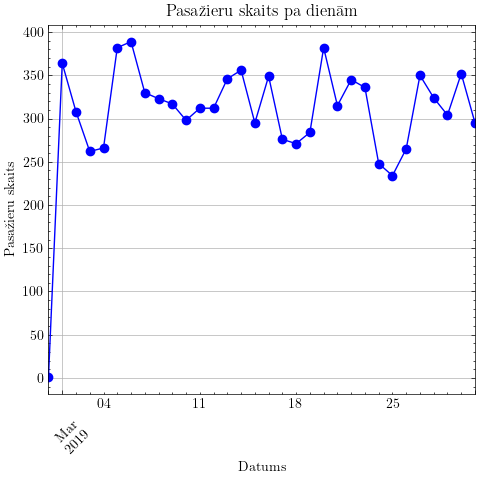
\includegraphics[width=0.65\textwidth]{6.uzd2.png}

\noindent \textbf{Piezīme:}
\begin{verbatim}
passengers_per_day = df['passengers'].resample('D').sum()
plt.figure(figsize=(5, 5))
passengers_per_day.plot(marker='o', linestyle='-', color='b')
plt.title('Pasažieru skaits pa dienām')
plt.xlabel('Datums')
plt.ylabel('Pasažieru skaits')
plt.grid(True)
plt.xticks(rotation=45)
plt.tight_layout()
plt.show()
\end{verbatim}
\subsection*{7. uzdevums.} Uzzīmēt grafikā brauciena vidējo ātrumu atkarībā no diennakts stundas.\\

\noindent \textbf{Atbilde}: 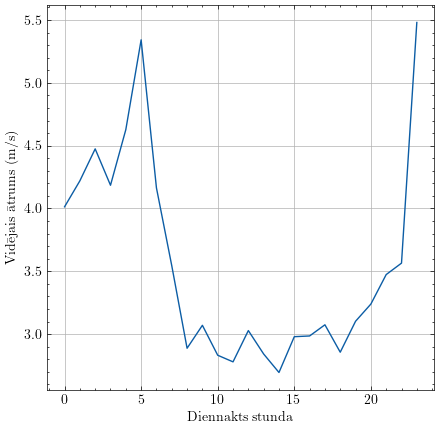
\includegraphics[width=0.5\textwidth]{7.uzd.png}

\noindent \textbf{Piezīme:}
\begin{verbatim}
mean_speed = df['mean_speed'].groupby(df.index.hour).mean()
plt.figure(figsize=(5, 5))
mean_speed.plot()
plt.xlabel('Diennakts stunda')
plt.ylabel('Vidējais ātrums (m/s)')
plt.grid(True)
plt.show()
\end{verbatim}
\subsection*{8. uzdevums.} Uzzīmēt grafikā vidējo brauciena ilgumu atkarībā no diennakts stundas.\\

\noindent \textbf{Atbilde:} 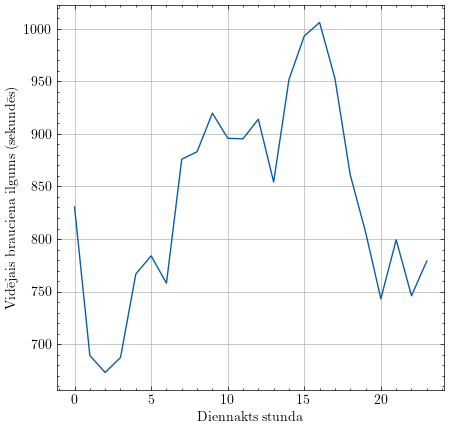
\includegraphics[width=0.5\textwidth]{8.uzd.png}

\noindent \textbf{Piezīme:}
\begin{verbatim}
distance_hour = df['time'].groupby(df.index.hour).mean()
plt.figure(figsize=(5, 5))
distance_hour.plot()
plt.xlabel('Diennakts stunda')
plt.ylabel('Vidējais brauciena ilgums (sekundēs)')
plt.grid(True)
plt.show()
\end{verbatim}
\subsection*{9. uzdevums.} Cik braucienu ir bijis katrā maršrutā? (apskatīt braucienu skaitu atkarībā no sākuma un beigu borough) \\
\textbf{Atbilde:} \begin{verbatim}
        ('Bronx', 'Bronx') 66
        ('Bronx', 'Brooklyn') 4
        ('Bronx', 'Manhattan') 25
        ('Bronx', 'Queens') 4
        ('Brooklyn', 'Bronx') 5
        ('Brooklyn', 'Brooklyn') 280
        ('Brooklyn', 'Manhattan') 67
        ('Brooklyn', 'Queens') 26
        ('Manhattan', 'Bronx') 54
        ('Manhattan', 'Brooklyn') 151
        ('Manhattan', 'Manhattan') 4857
        ('Manhattan', 'Queens') 162
        ('Manhattan', 'Staten Island') 2
        ('Queens', 'Bronx') 11
        ('Queens', 'Brooklyn') 62
        ('Queens', 'Manhattan') 223
        ('Queens', 'Queens') 342
        route count = 17
        num route = 6341
\end{verbatim}

\noindent \textbf{Piezīme:}
\begin{verbatim}
# all possible routes
routes = df.groupby(['pickup_borough', 'dropoff_borough']).size()
routes_count = []

for route in routes.index:
    print(route, routes[route])
    routes_count.append(routes[route])

print(np.count_nonzero(routes_count))
print(np.sum(routes_count))
\end{verbatim}
\subsection*{10. uzdevums.} Atlasīt tikai tos gadījumus, kad brauciena attālums lielāks par 0 (lai izvairītos no kļūdas). Kāda ir vidējā brauciena cena par kilometru atkarībā no diennakts stundas?\\
\textbf{Atbilde:} 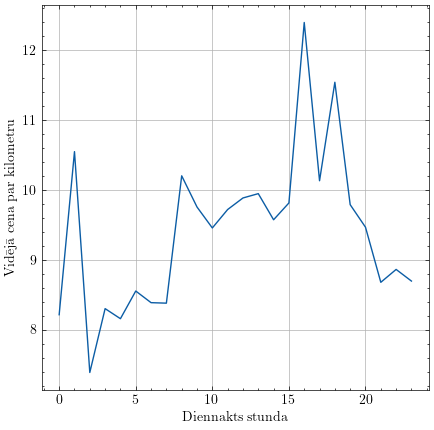
\includegraphics[width=0.5\textwidth]{10.uzd..png}

\noindent \textbf{Piezīme:}
\begin{verbatim}
df_filtered = df[df.distance > 0]
price_per_km_bigger_o = df_filtered['fare_per_kilometre'].
groupby(df_filtered.index.hour).mean()

plt.figure(figsize=(5, 5))
price_per_km_bigger_o.plot()
plt.xlabel('Diennakts stunda')
plt.ylabel('Vidējā cena par kilometru')
plt.grid(True)
plt.show()
\end{verbatim}
\subsection*{11. uzdevums.} Cik braucienu, kas garumā starp 5 km un 10 km, ir notikuši?\\
\textbf{Atbilde:} 554

\noindent \textbf{Piezīme:}
\begin{verbatim}
df_filtr = df[(df.distance > 5) & (df.distance < 10)]
count = df_filtr['distance'].count()
print(count)
\end{verbatim}
\subsection*{12. uzdevums.} Uzzīmēt pasažieru kopējo skaitu pa dienām, kuri sāk braucienu \textit{Manhattan}.\\
\textbf{Atbilde:} 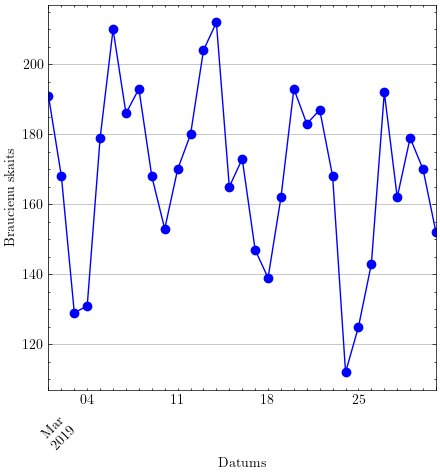
\includegraphics[width=0.5\textwidth]{12.udz.png}

\noindent \textbf{Piezīme:}
\begin{verbatim}
manhetenas_skaits = df[df.pickup_borough == 'Manhattan'].resample('D').size()
manhetenas_skaits.plot(figsize=(5, 5), marker='o', linestyle='-', color='b')
plt.ylabel('Braucienu skaits')
plt.xlabel('Datums')
plt.grid(True)
plt.xticks(rotation=45)
plt.show()
\end{verbatim}
\subsection*{13. uzdevums.} Atlasīt tikai tos braucienus, kam sākuma un beigu borough sakrīt. Kāds ir vidējais brauciena ilgums katra borough robežās?\\
\textbf{Atbilde:} \begin{table}[ht]
\centering
\begin{tabular}{ccc}
\hline
 & Borough   & Average Trip Duration (minutes) \\ \hline
0     & Bronx     & 18.28636363636364              \\
1     & Brooklyn  & 14.642559523809524             \\
2     & Manhattan & 11.460191476219888             \\
3     & Queens    & 11.845808966861599             \\ \hline
\end{tabular}
\label{tab:trip_duration}
\end{table}

\noindent \textbf{Piezīme:}
\begin{verbatim}
same_borough_trips = df[df['pickup_borough'] == df['dropoff_borough']]

average_trip_duration = same_borough_trips.groupby('pickup_borough')['time_minutes'].mean()
print(average_trip_duration)
\end{verbatim}
\subsection*{14. uzdevums.} Uzzīmēt diennakts vidējo pasažieru skaitu atkarībā no nedēļas dienas.\\
\textbf{Atbilde:} 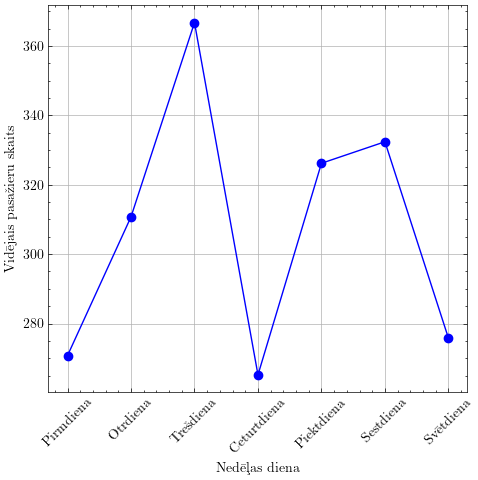
\includegraphics[width=0.5\textwidth]{14.uzd.png}

\noindent \textbf{Piezīme:}
\begin{verbatim}
average_passengers_by_weekday = passengers_per_day.groupby(passengers_per_day.index.
dayofweek).mean()
average_passengers_by_weekday.index = dienas

plt.figure(figsize=(5, 5))
plt.plot(average_passengers_by_weekday.index, average_passengers_by_weekday.values,
             marker='o', linestyle='-', color='b')
plt.xlabel('Nedēļas diena')
plt.ylabel('Vidējais pasažieru skaits')
plt.grid(True)
plt.xticks(rotation=45)
plt.tight_layout()
plt.show()
\end{verbatim}
\subsection*{15. uzdevums.} Uzzīmēt grafikā vidējo braucienu skaitu atkarībā no diennakts stundas.\\
\textbf{Atbilde:} 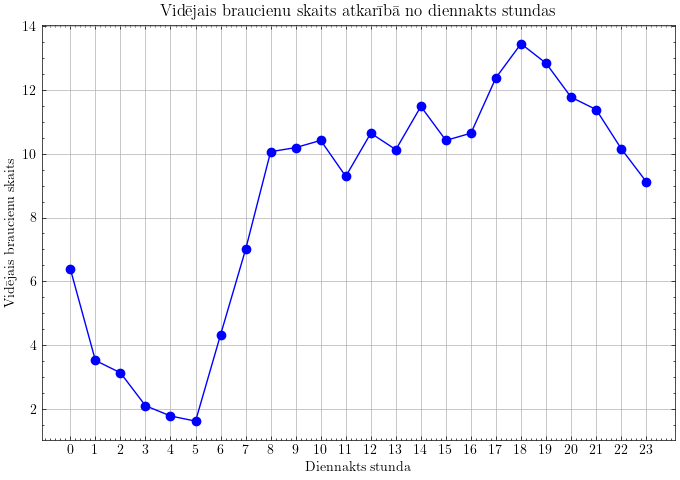
\includegraphics[width=0.7\textwidth]{15.uzd.png}

\noindent \textbf{Piezīme:}
\begin{verbatim}
average_trips_per_hour = df.resample('H').size().groupby(df.resample('H').size().index.hour).mean()

plt.figure(figsize=(7, 5))
average_trips_per_hour.plot(marker='o', linestyle='-', color='b')
plt.xlabel('Diennakts stunda')
plt.ylabel('Vidējais braucienu skaits')
plt.title('Vidējais braucienu skaits atkarībā no diennakts stundas')
plt.grid(True)
plt.xticks(range(24))
plt.tight_layout()
plt.show()
\end{verbatim}
\subsection*{16. uzdevums.} Atlasīt tikai tos braucienus, kam sākuma un beigu borough sakrīt. Atlasīt tikai tos gadījumus, kad brauciena attālums lielāks par 0 (lai izvairītos no kļūdas). Kāda ir vidējā brauciena cena par kilometru katrā no borough? \\
\textbf{Atbilde:} \begin{table}[ht]
\centering
\begin{tabular}{lc}
\hline
Borough    & Average Ride Price per km \\ \hline
Bronx      & 7.50                      \\
Brooklyn   & 7.44                      \\
Manhattan  & 10.71                     \\
Queens     & 9.22                      \\ \hline
\end{tabular}
\label{tab:ride_price}
\end{table}

\noindent \textbf{Piezīme:}
\begin{verbatim}
df_same = df[(df.pickup_borough == df.dropoff_borough)*(df.distance > 0)]

avg_fare_per_km = df_same.groupby("pickup_borough")["fare_per_kilometre"].mean()

print(avg_fare_per_km)
\end{verbatim}
\end{document}
